\documentclass[12pt, letterpaper]{article}
\usepackage[utf8]{inputenc}
\usepackage[margin=1in]{geometry}
\usepackage[super]{nth}
\usepackage{hyperref}
\usepackage{lineno}
\usepackage[
singlelinecheck=false
]{caption}
\usepackage{amsmath}
\usepackage{amsfonts}
\usepackage{bm}
\usepackage{bbm}
\usepackage{graphicx}
\usepackage{csvsimple}
\usepackage[section]{placeins}
\usepackage{lineno}
\usepackage{natbib}

\title{A joint framework for PCA and F-statistics}
\author{Divyaratan Popli, Benjamin M. Peter}
%\date{5 August 2021}
\linenumbers

\setlength{\parskip}{1em}
\setlength{\parindent}{0em}

\newcommand{\BZ}{\mathbf{Z}}
\newcommand{\BD}{\mathbf{D}}
\newcommand{\BN}{\mathbf{N}}
\newcommand{\BH}{\mathbf{H}}
\newcommand{\Btheta}{\pmb{\theta}}


\begin{document}

\maketitle
%\renewcommand\thefigure{\arabic{figure}}    
\section*{Supplementary Figures}
%\setcounter{figure}{0}   
\renewcommand{\figurename}{Fig S}

\begin{figure}[ht!]
    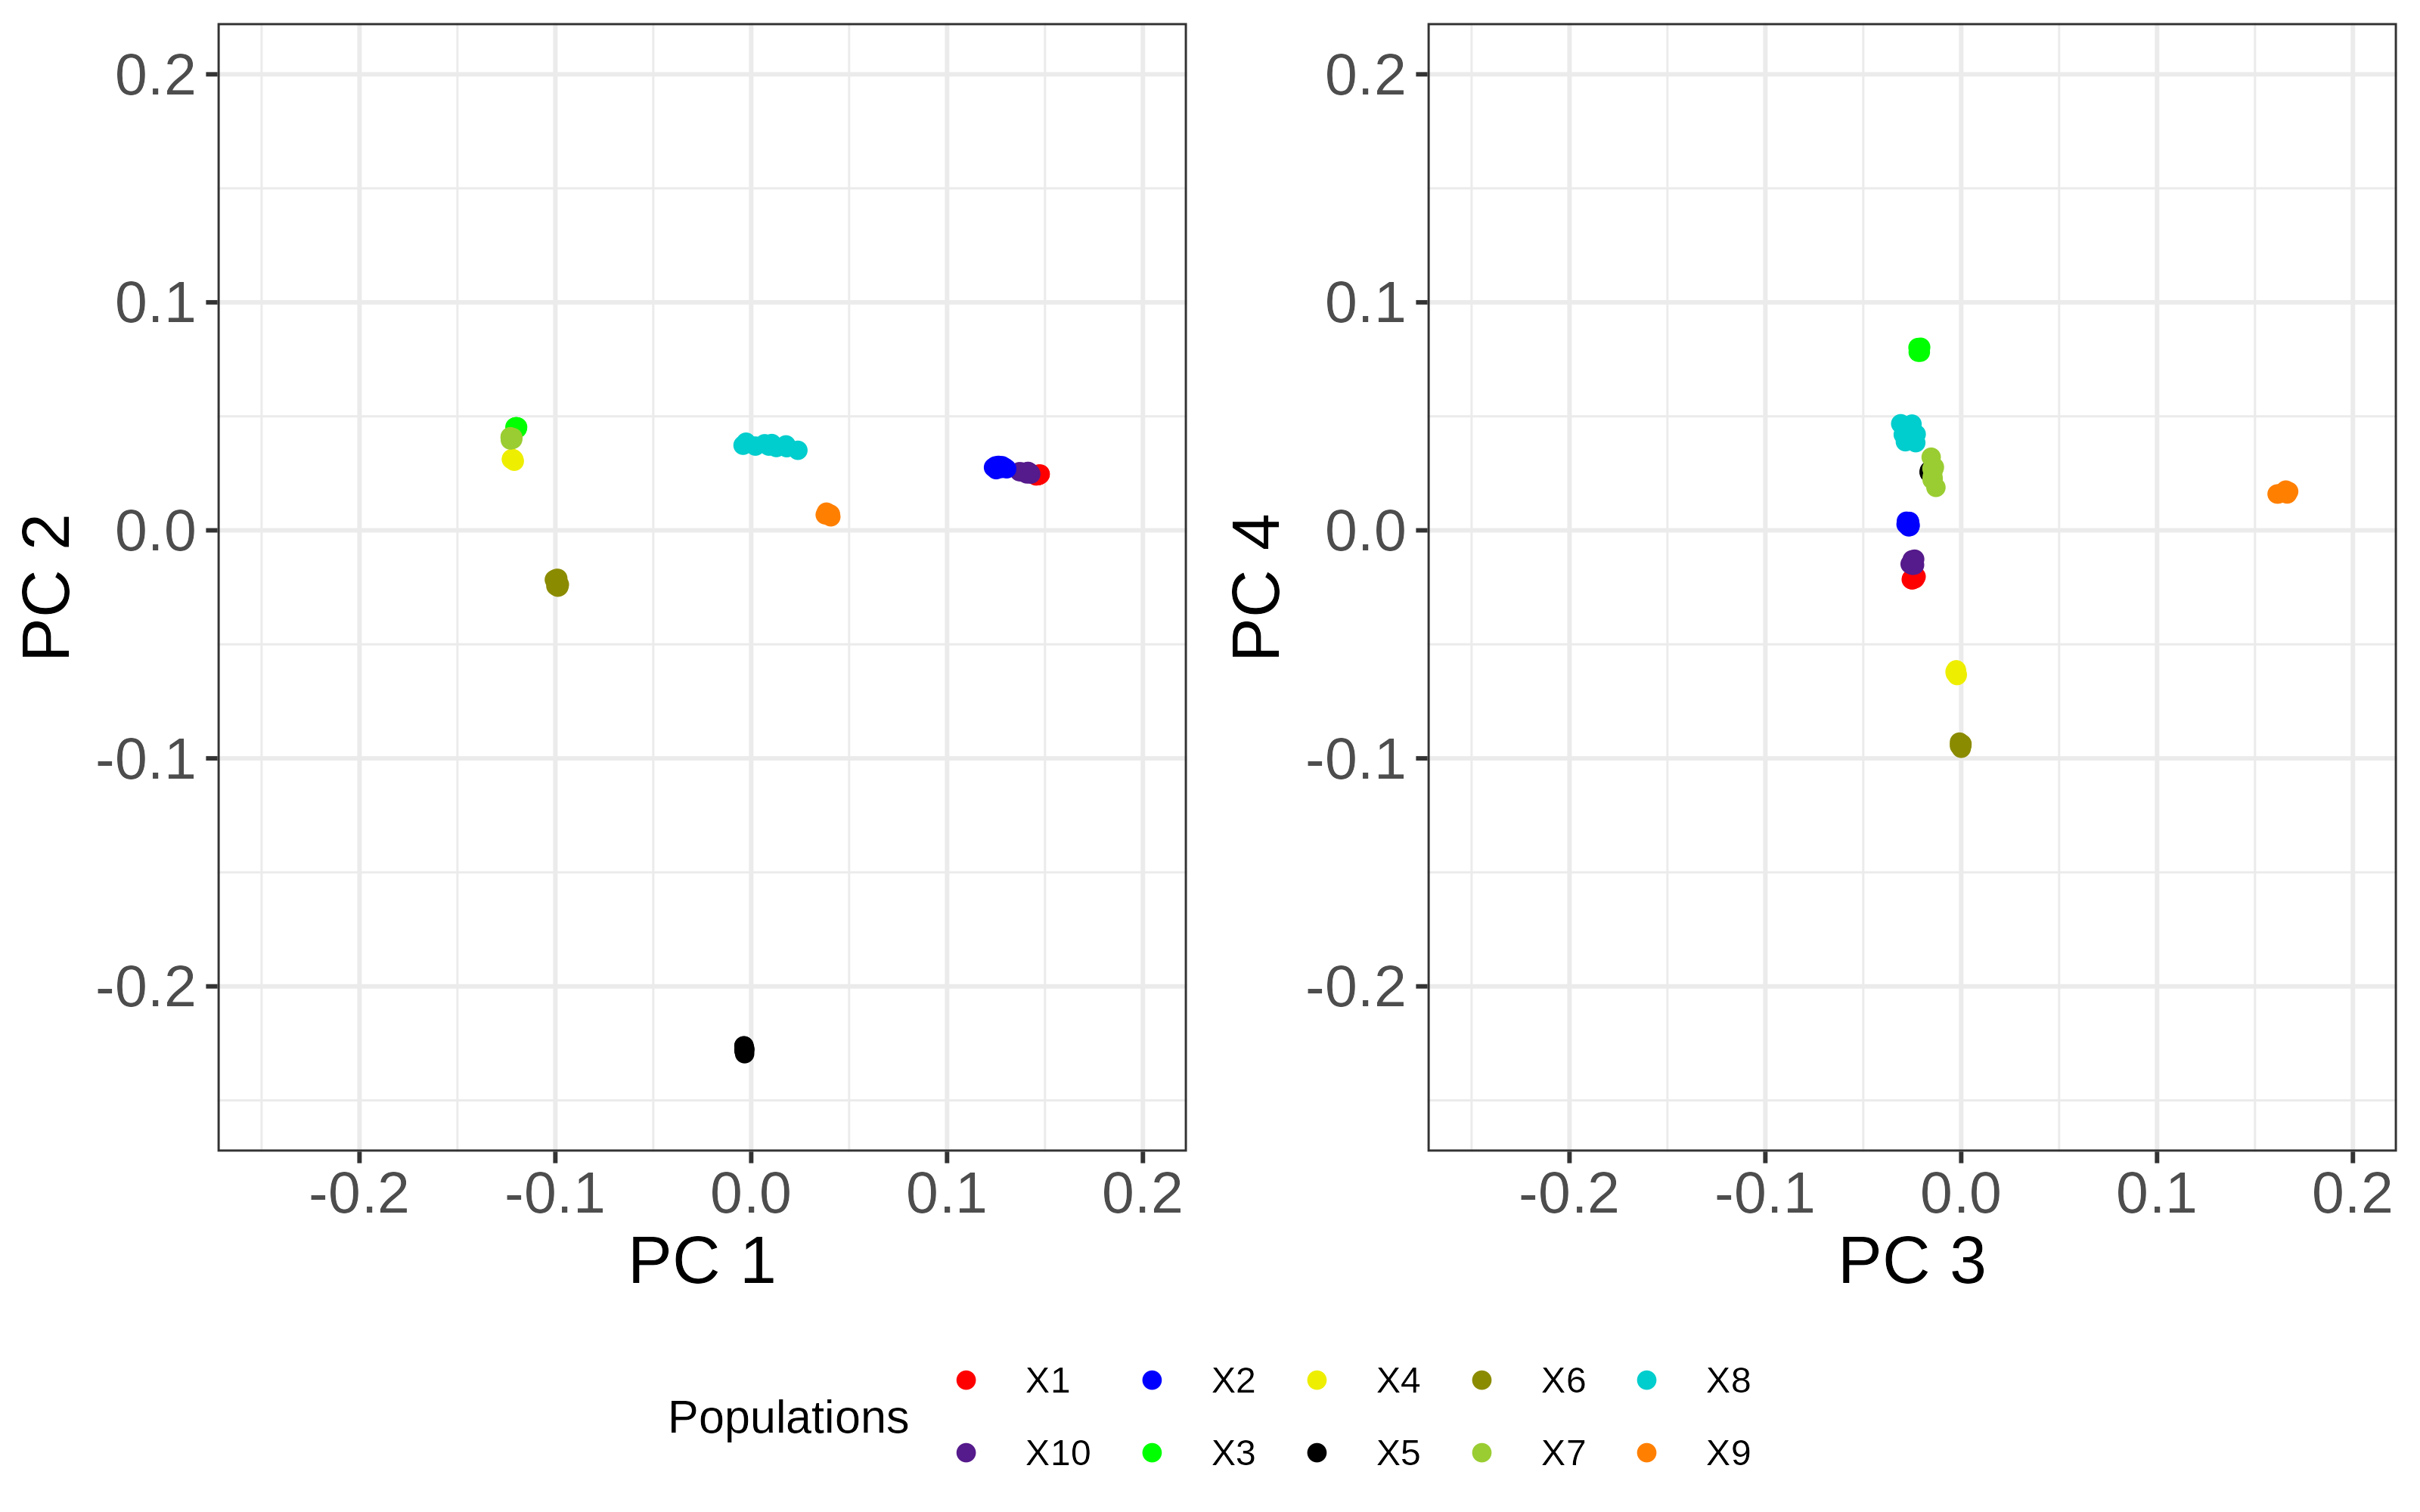
\includegraphics[width=16.5cm]{plots/supplementary/pcplot1.png}
    \centering
    \caption{PPCA (scale=8) reveals population structure, similar to a PCA plot. Data is taken from simulations with phylogenetic tree shown in Fig. 2A.}
    \label{figS1:pc_scale}
\end{figure}


\begin{figure}[ht!]
    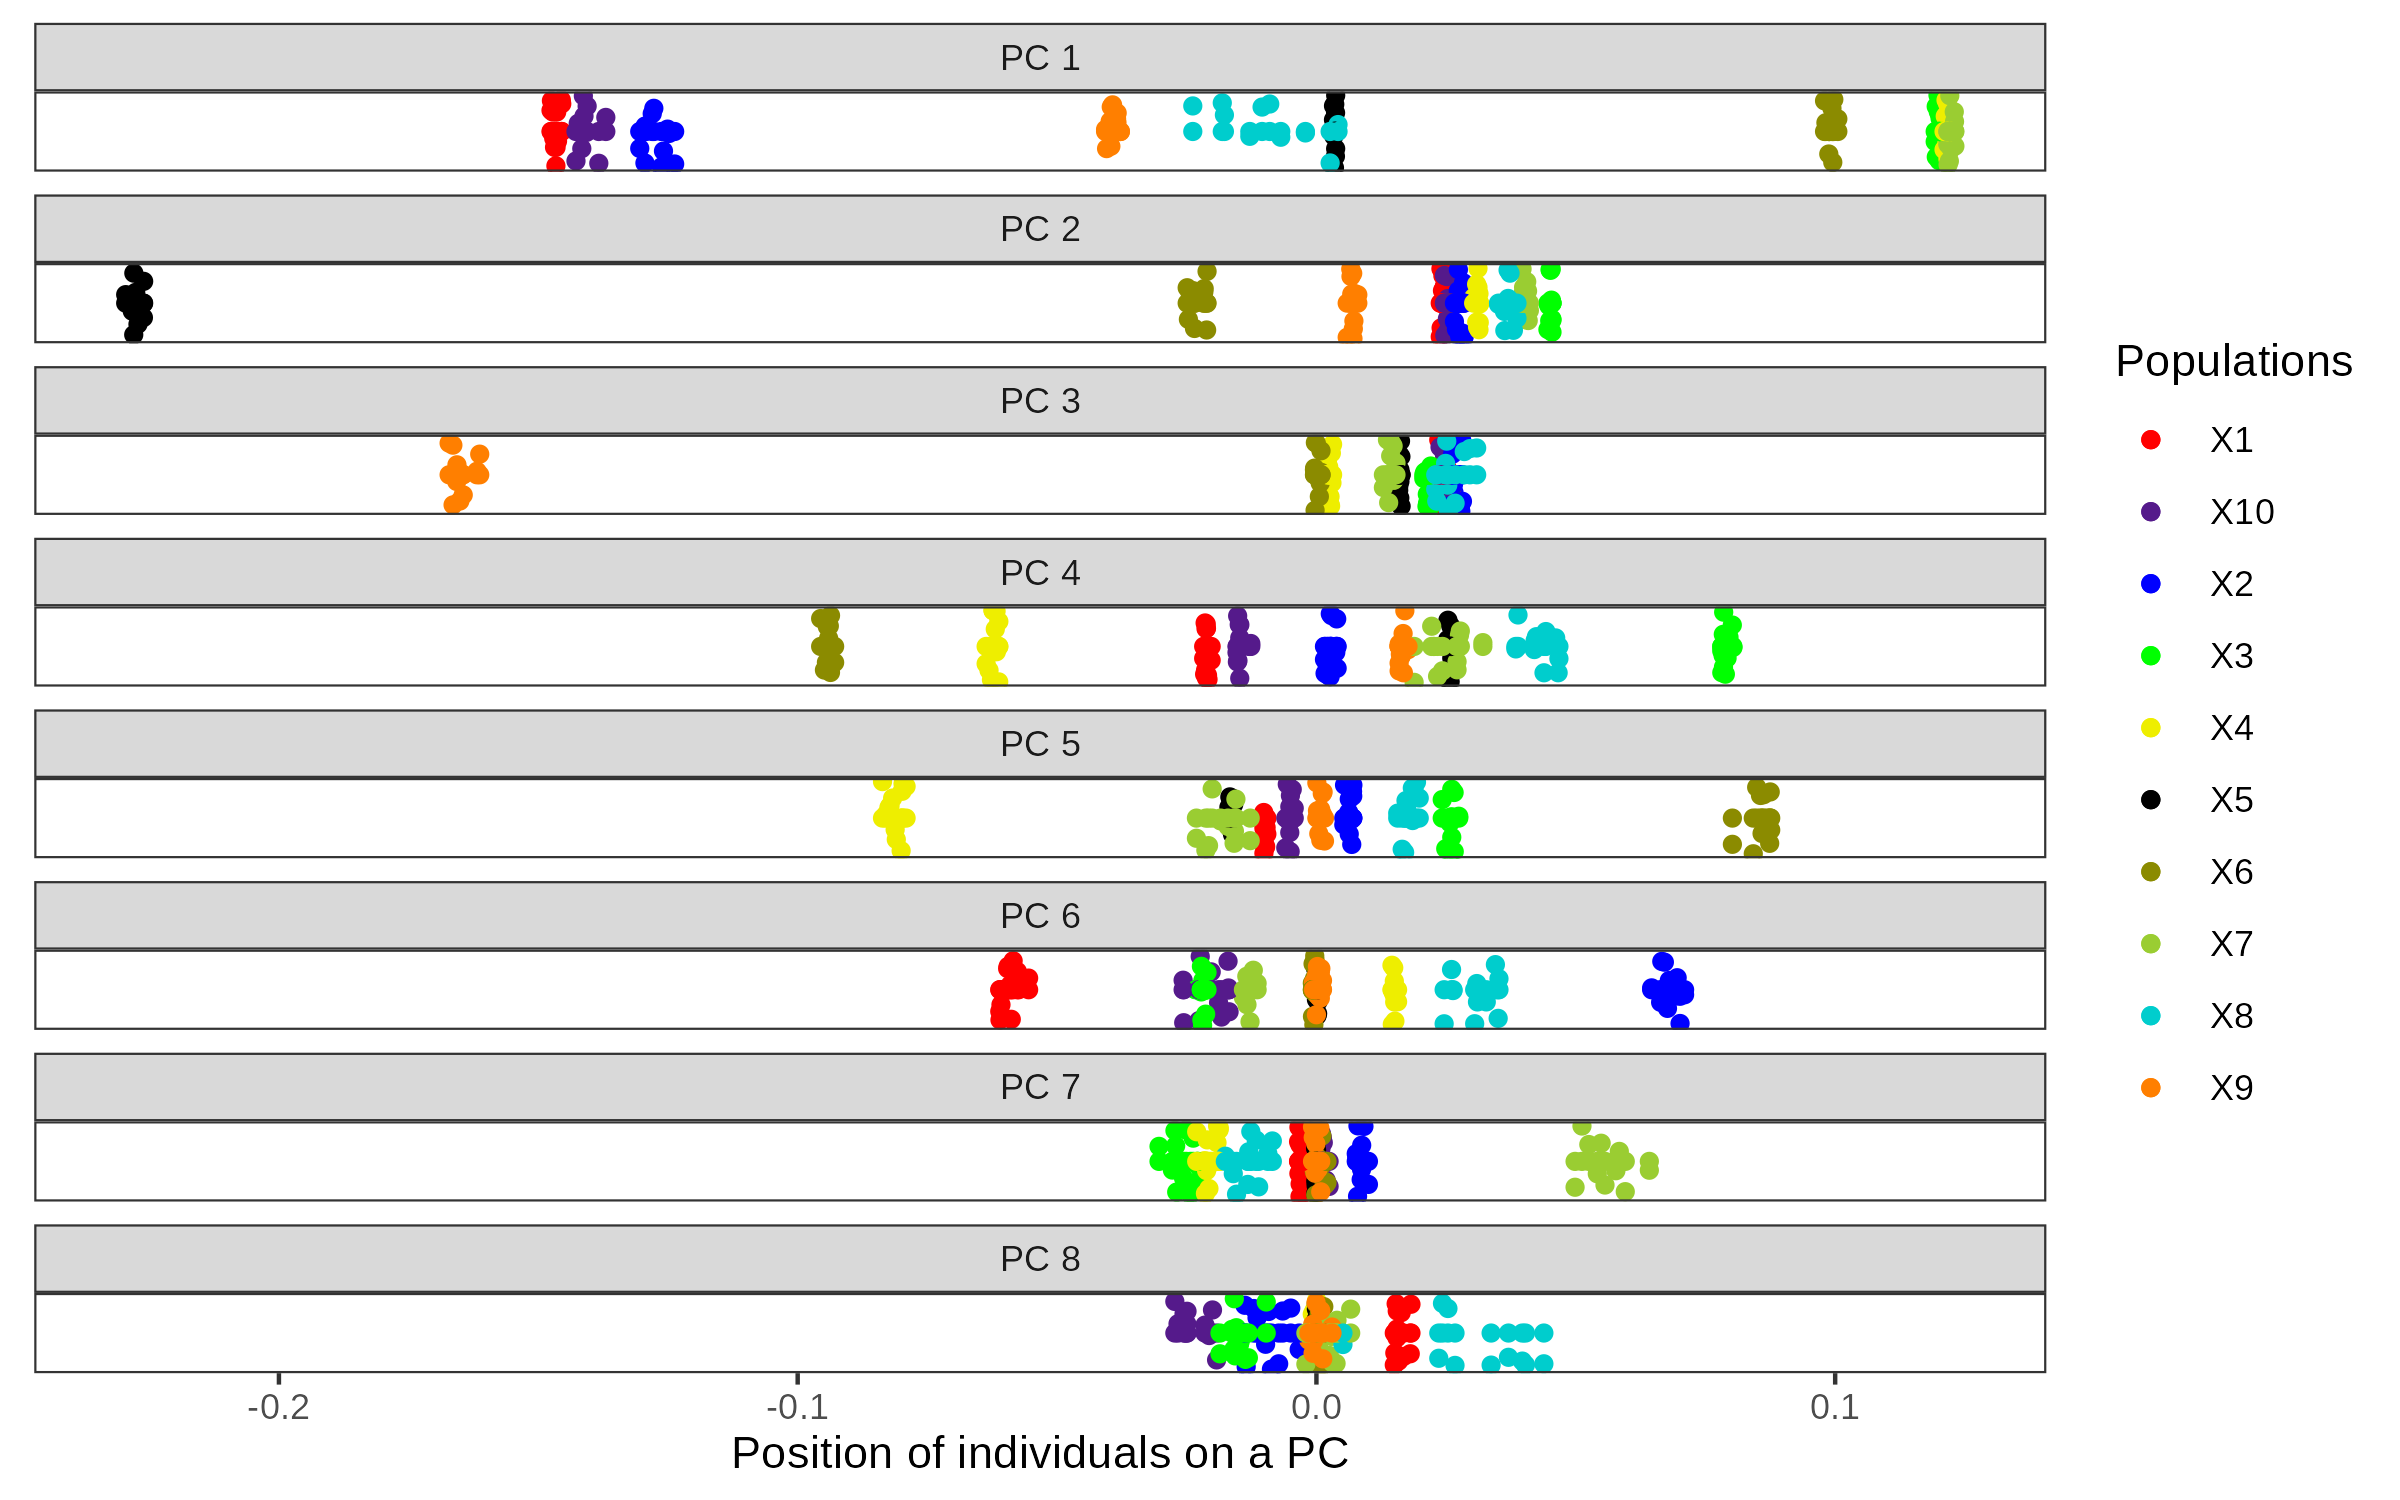
\includegraphics[width=16.5cm]{plots/supplementary/pcplot2.png}
    \centering
    \caption{Variation in the genetic data explained with the top 8 PCs from PPCA. Each panel shows the position of individuals on a Principal Component. Jitter is added to y-axis to show the data points clearly. The 10 PCs explain $27.21\%$, $19.37\%$, $13.82\%$, $12.2\%$ , $10.07\%$,  $8.33\%$,  $5.31\%$,  $3.68\%$, $0\%$ and $0\%$ variation in the data respectively. The last 2 PCs explain $0\%$ variation because the PPCA model with scale=8 explicitly sets the non- relevant PCs to 0.}
    \label{figS1:pc_scale}
\end{figure}

\begin{figure}[ht!]
    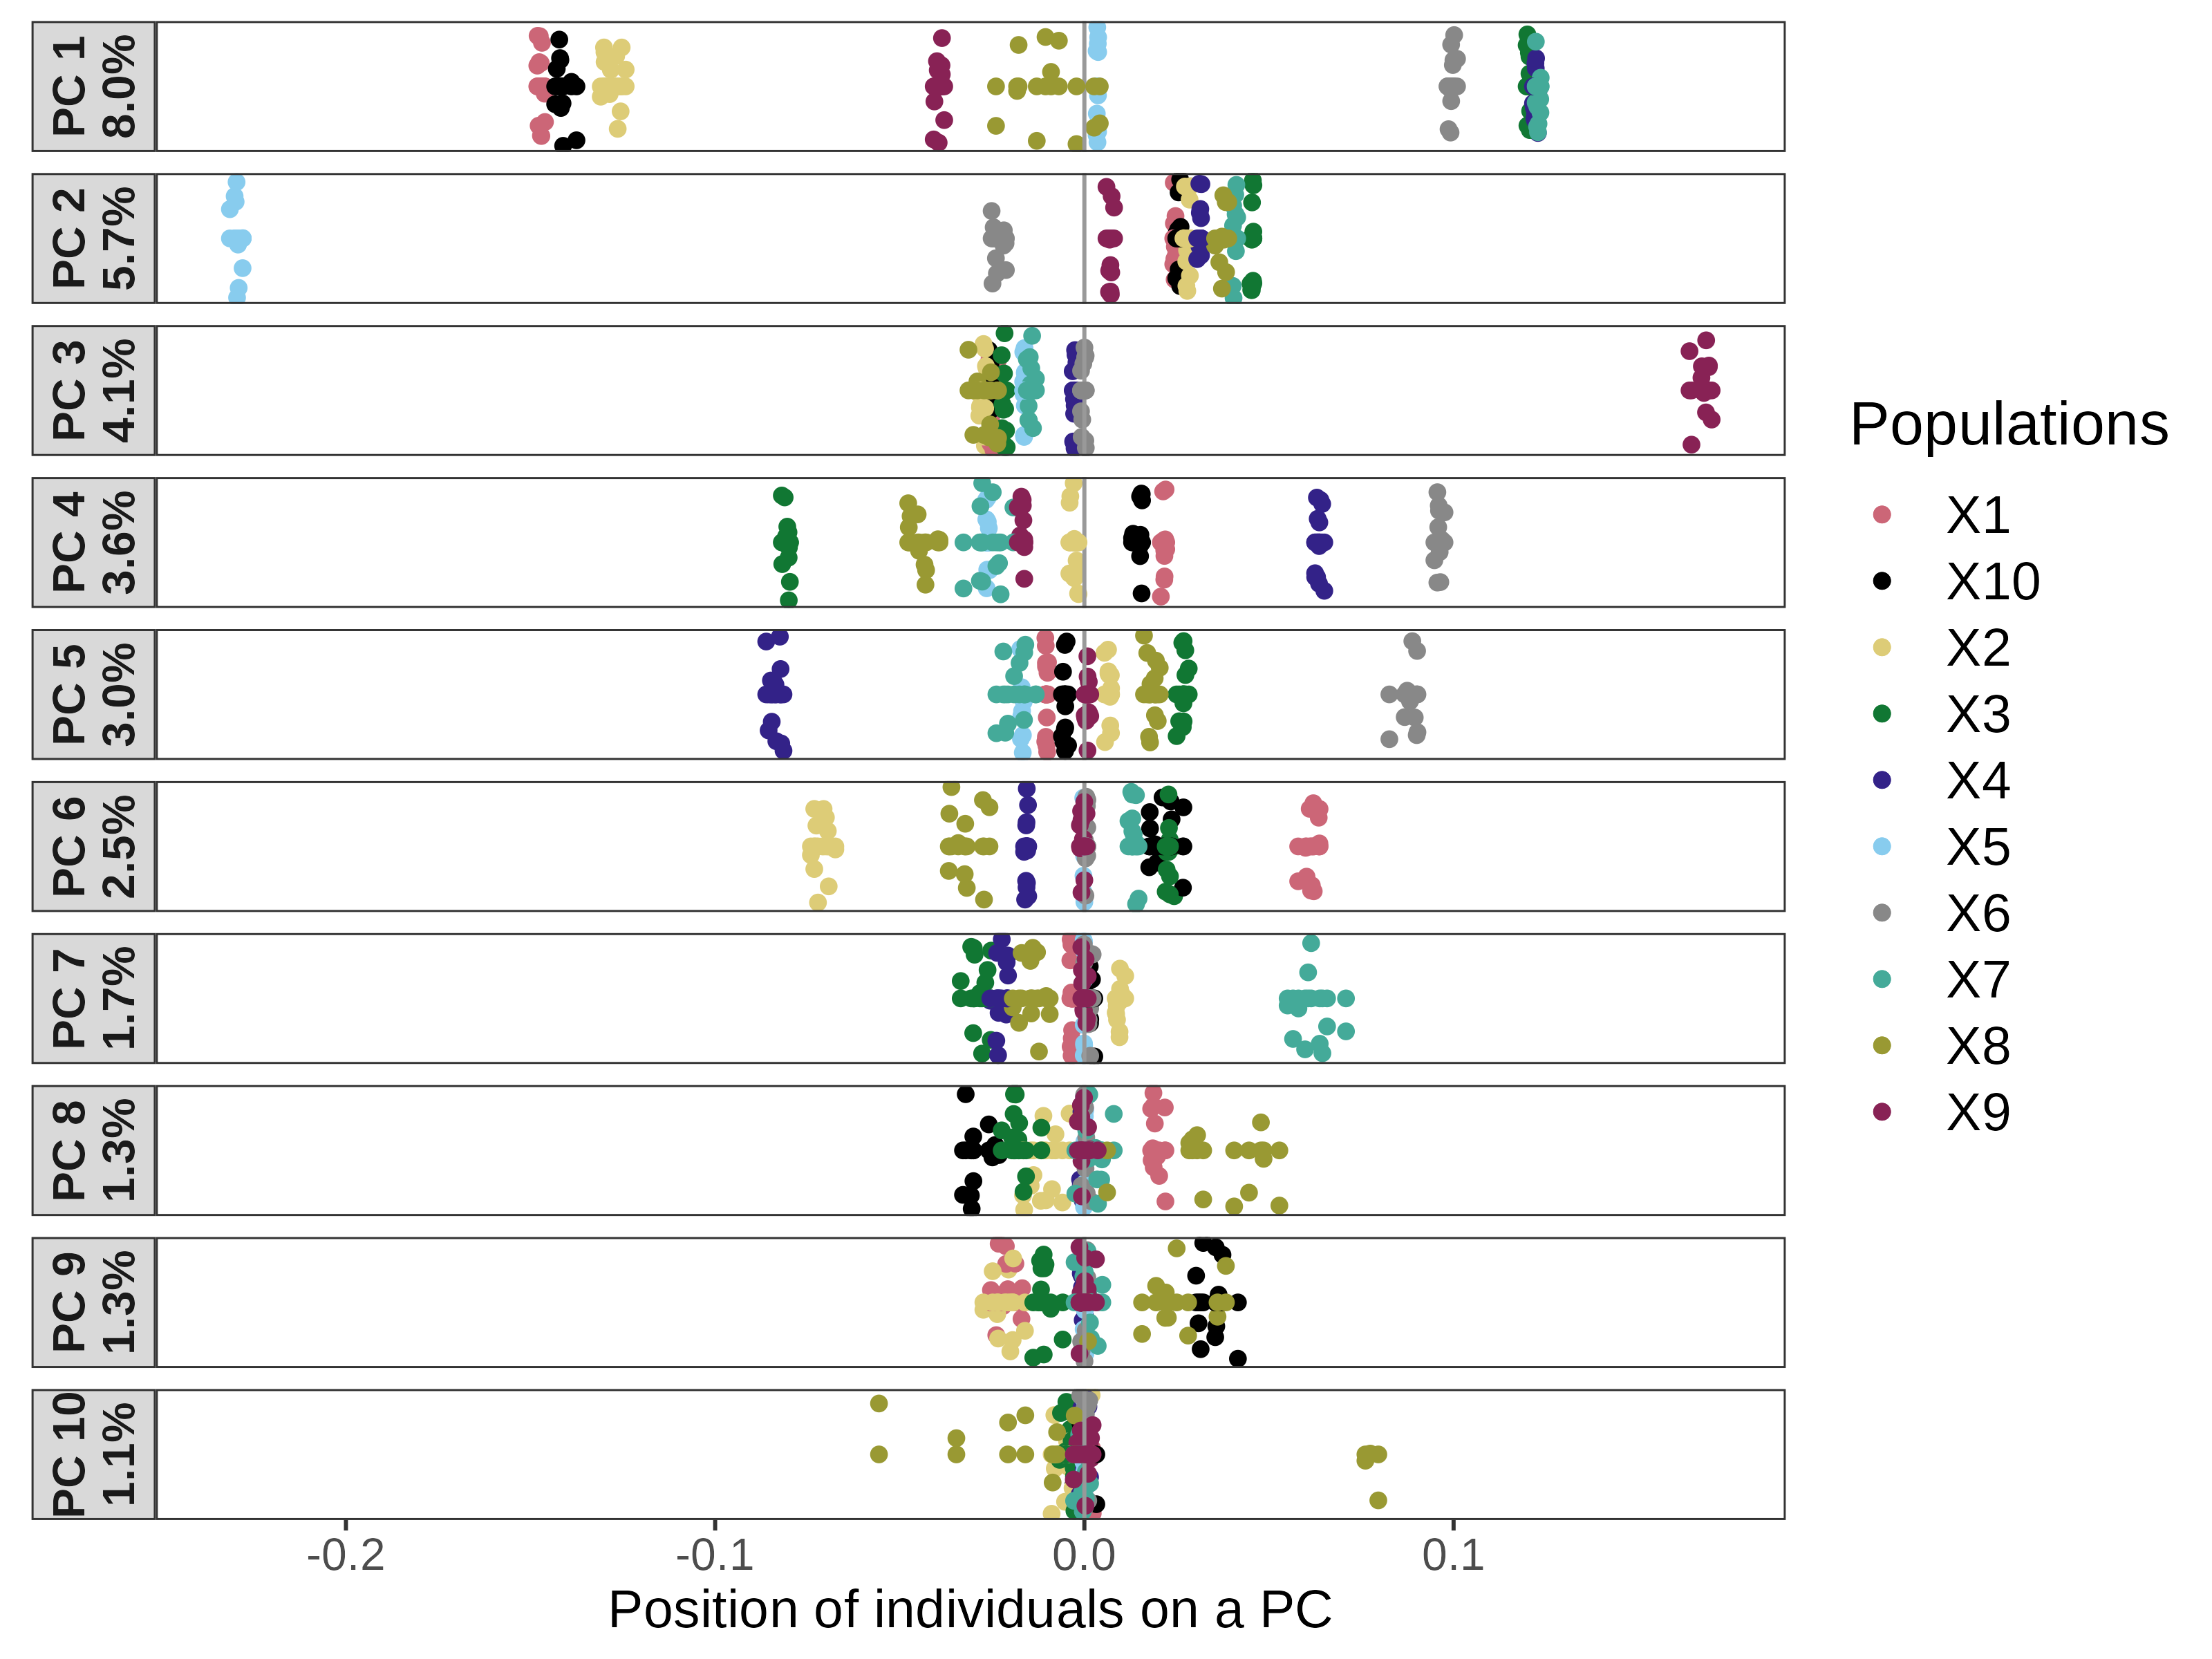
\includegraphics[width=16.5cm]{plots/supplementary/pcaplot2.png}
    \centering
    \caption{Variation in the genetic data explained with the top 8 PCs from PCA. Each panel shows the position of individuals on a Principal Component. Jitter is added to y-axis to show the data points clearly. The 10 PCs explain $7.99\%$, $5.72\%$, $4.11\%$, $3.65\%$, $3.04\%$, $2.55\%$, $1.72\%$, $1.31\%$, $1.26\%$, $1.12\%$ variation in the data respectively.}
    \label{figS1:pc_scale}
\end{figure}

\begin{figure}[ht!]
    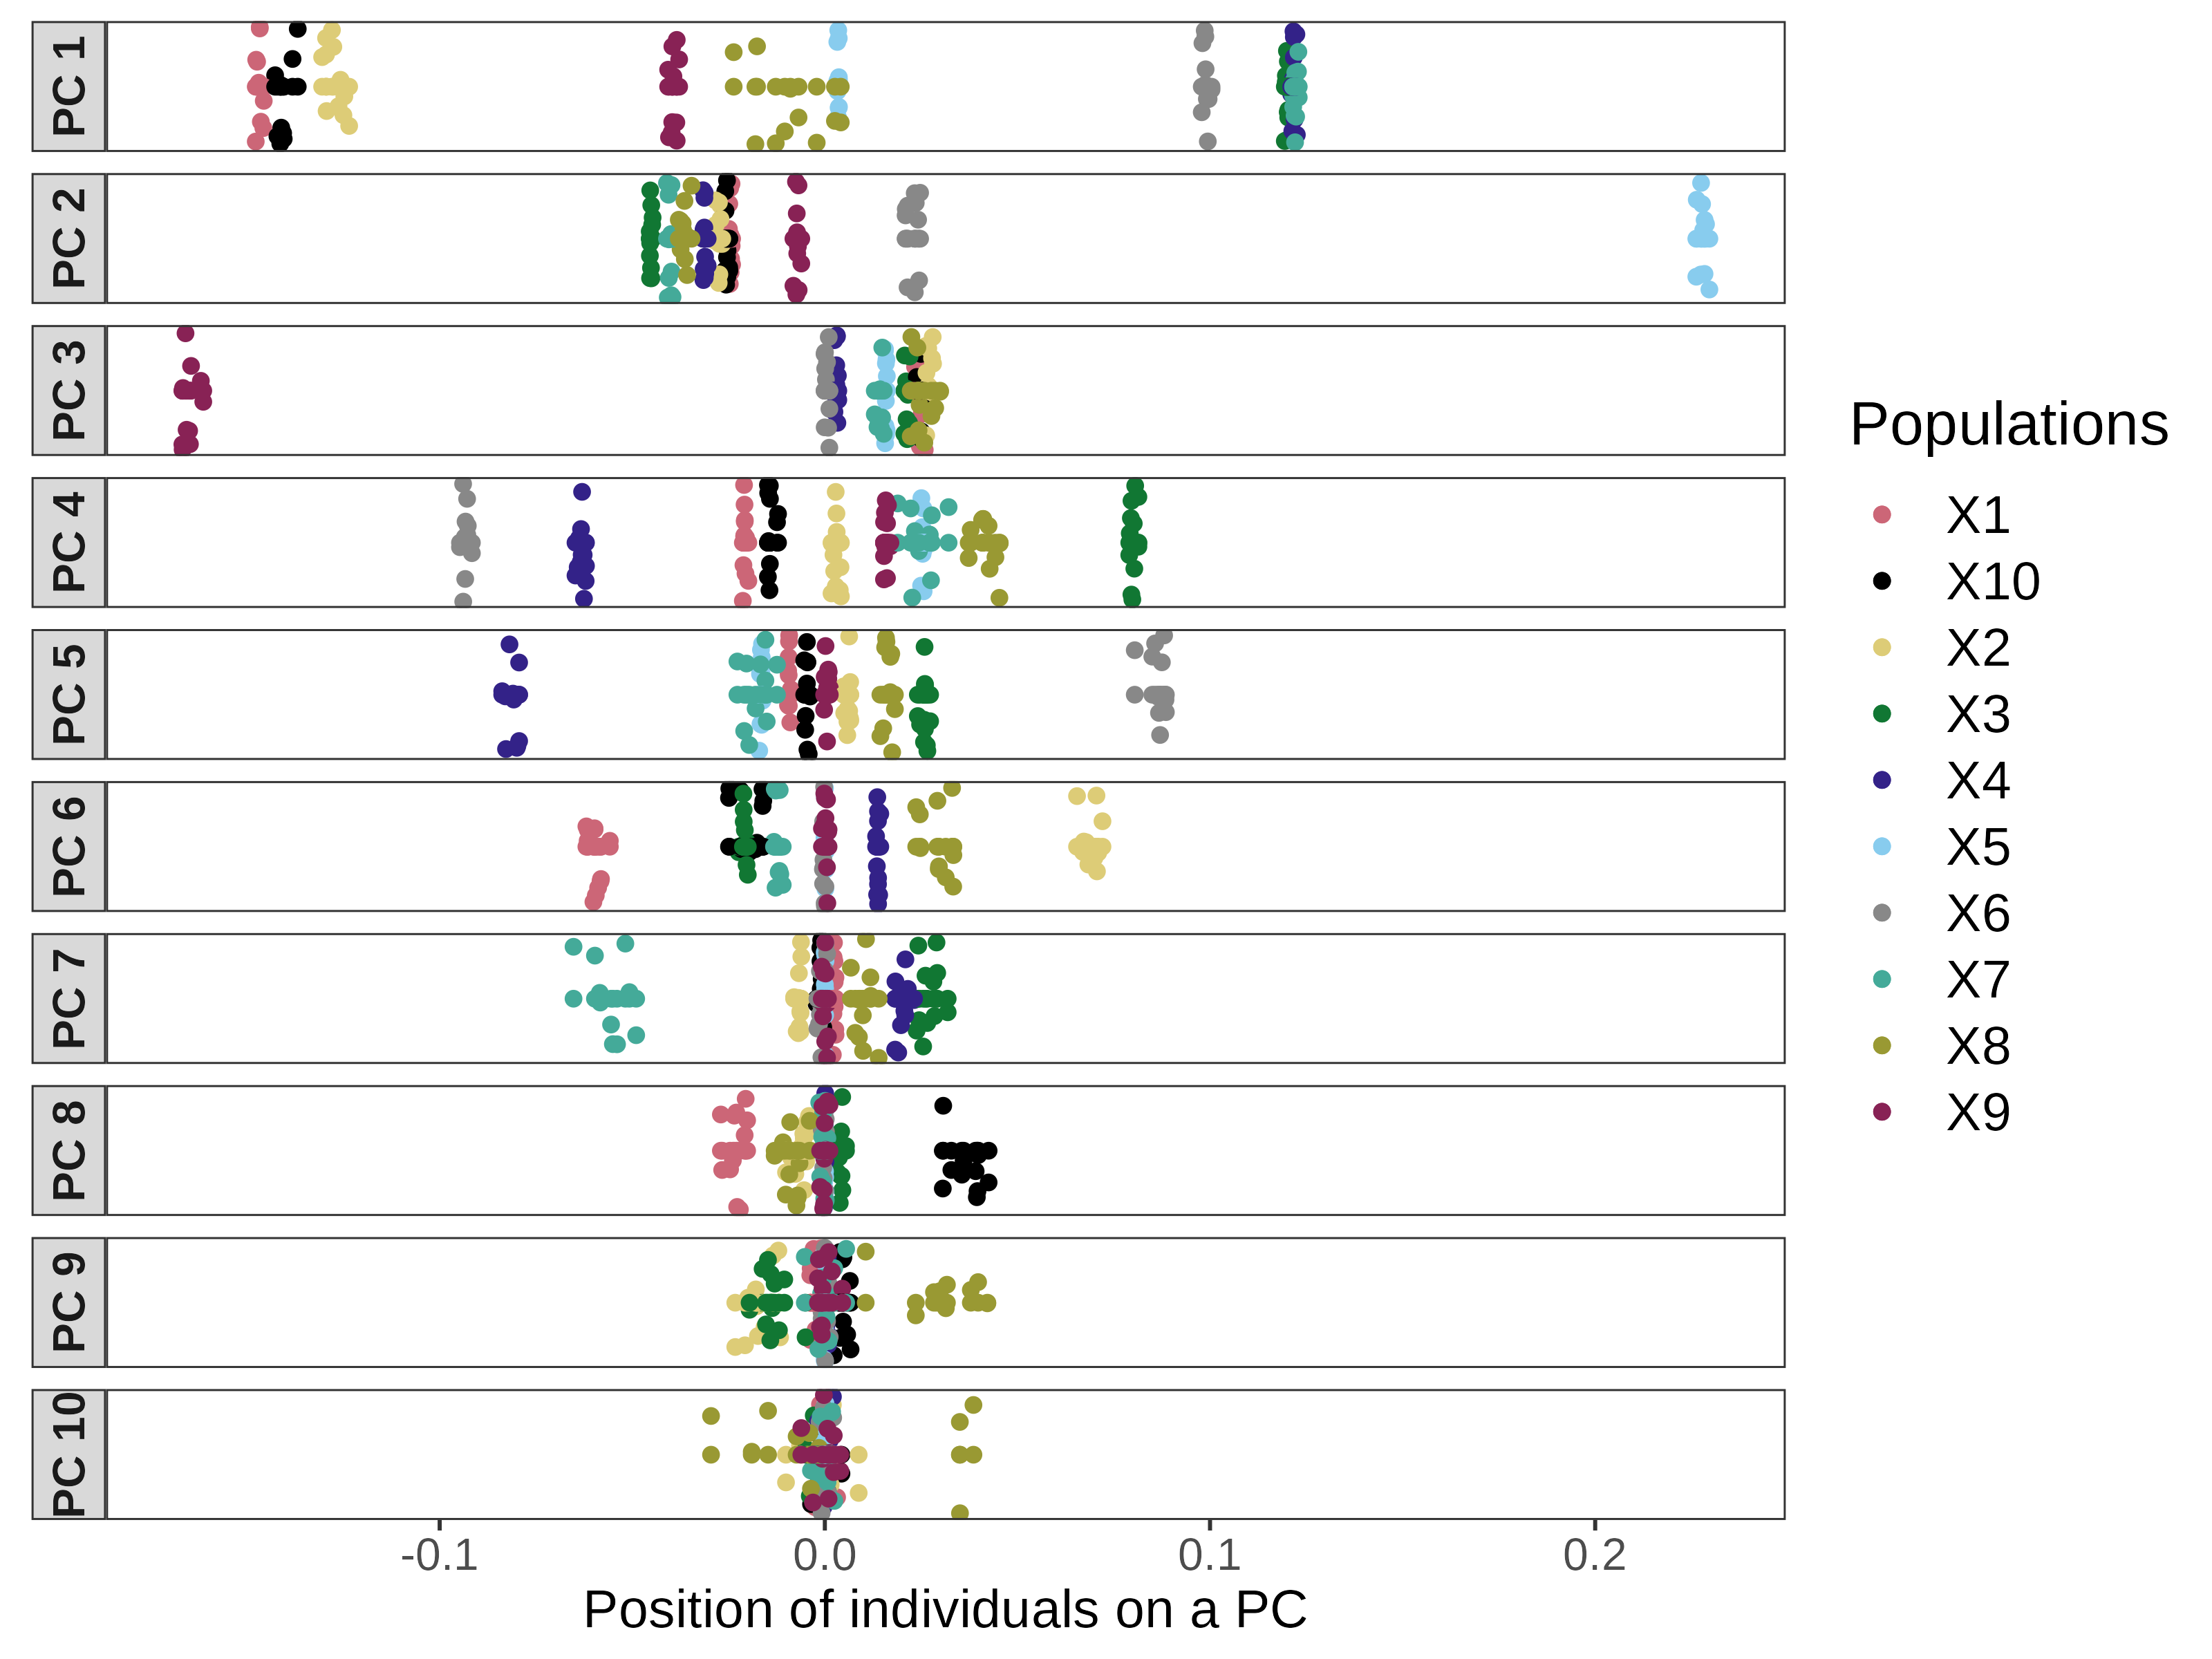
\includegraphics[width=16.5cm]{plots/supplementary/lseplot2.png}
    \centering
    \caption{Variation in the genetic data explained with the top 8 PCs from LSE. Each panel shows the position of individuals on a Principal Component. Jitter is added to y-axis to show the data points clearly. The 10 PCs explain $44.35\%$, $22.52\%$, $11.44\%$,  $8.92\%$,  $6.1\%$ ,  $4.16\%$,  $1.69\%$,  $0.77\%$,  $0.58\%$ and $0.22\%$ variation in the data respectively.}
    \label{figS1:pc_scale}
\end{figure}


\begin{figure}[ht!]
    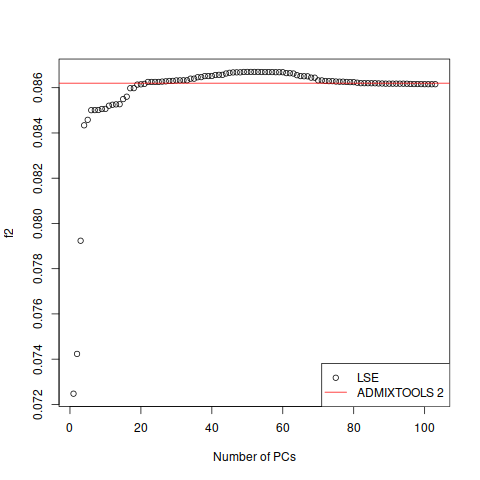
\includegraphics[width=16.5cm]{plots/supplementary/lse_admix.png}
    \centering
    \caption{$F_2(X_1,X_4)$ estimate from LSE converges to the estimate from ADMIXTOOLS 2, when all PCs are used.}
    \label{figS1:pc_scale}
\end{figure}


\begin{figure}[ht!]
    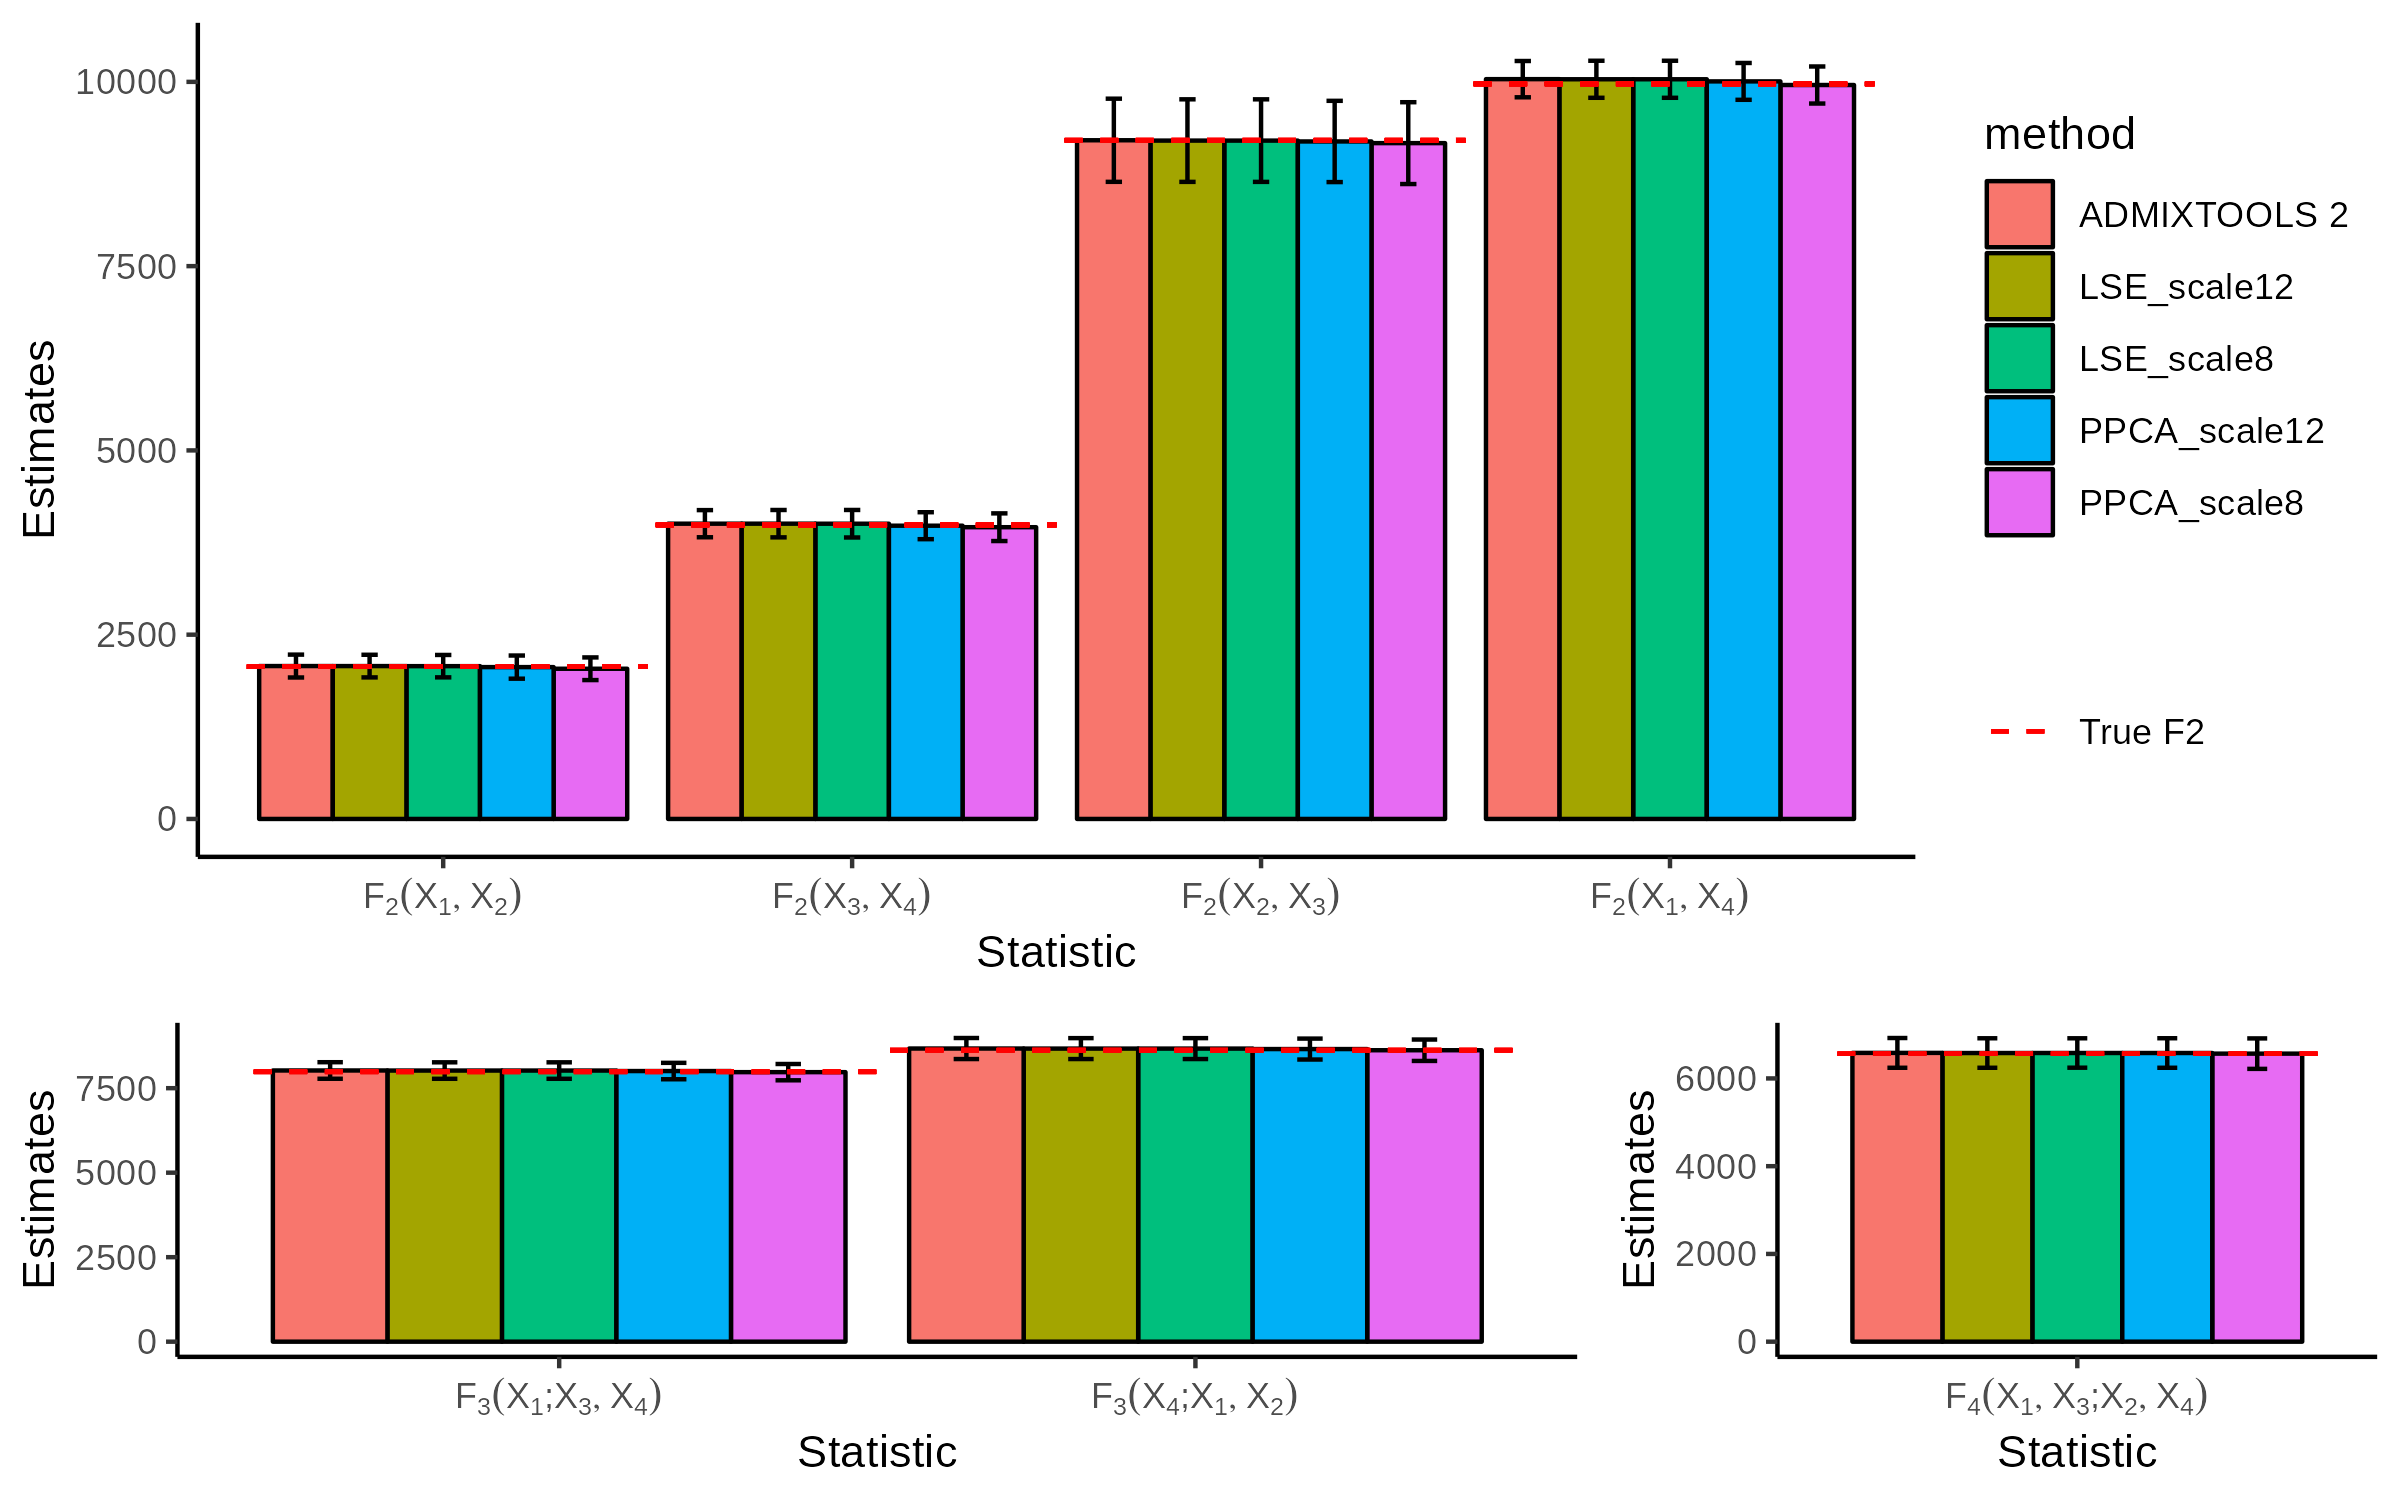
\includegraphics[width=16.5cm]{plots/simfiles/Ne1000/split_times1000/npop10_nind100/plots_8_12/mu0.05_plot_all.png}
    \centering
    \caption{Comparison of PPCA and LSE to ADMIXTOOLS 2 using population genotypes from ten individuals in each population.}
    \label{figS2:pc_scale}
\end{figure}

\begin{figure}[ht!]
    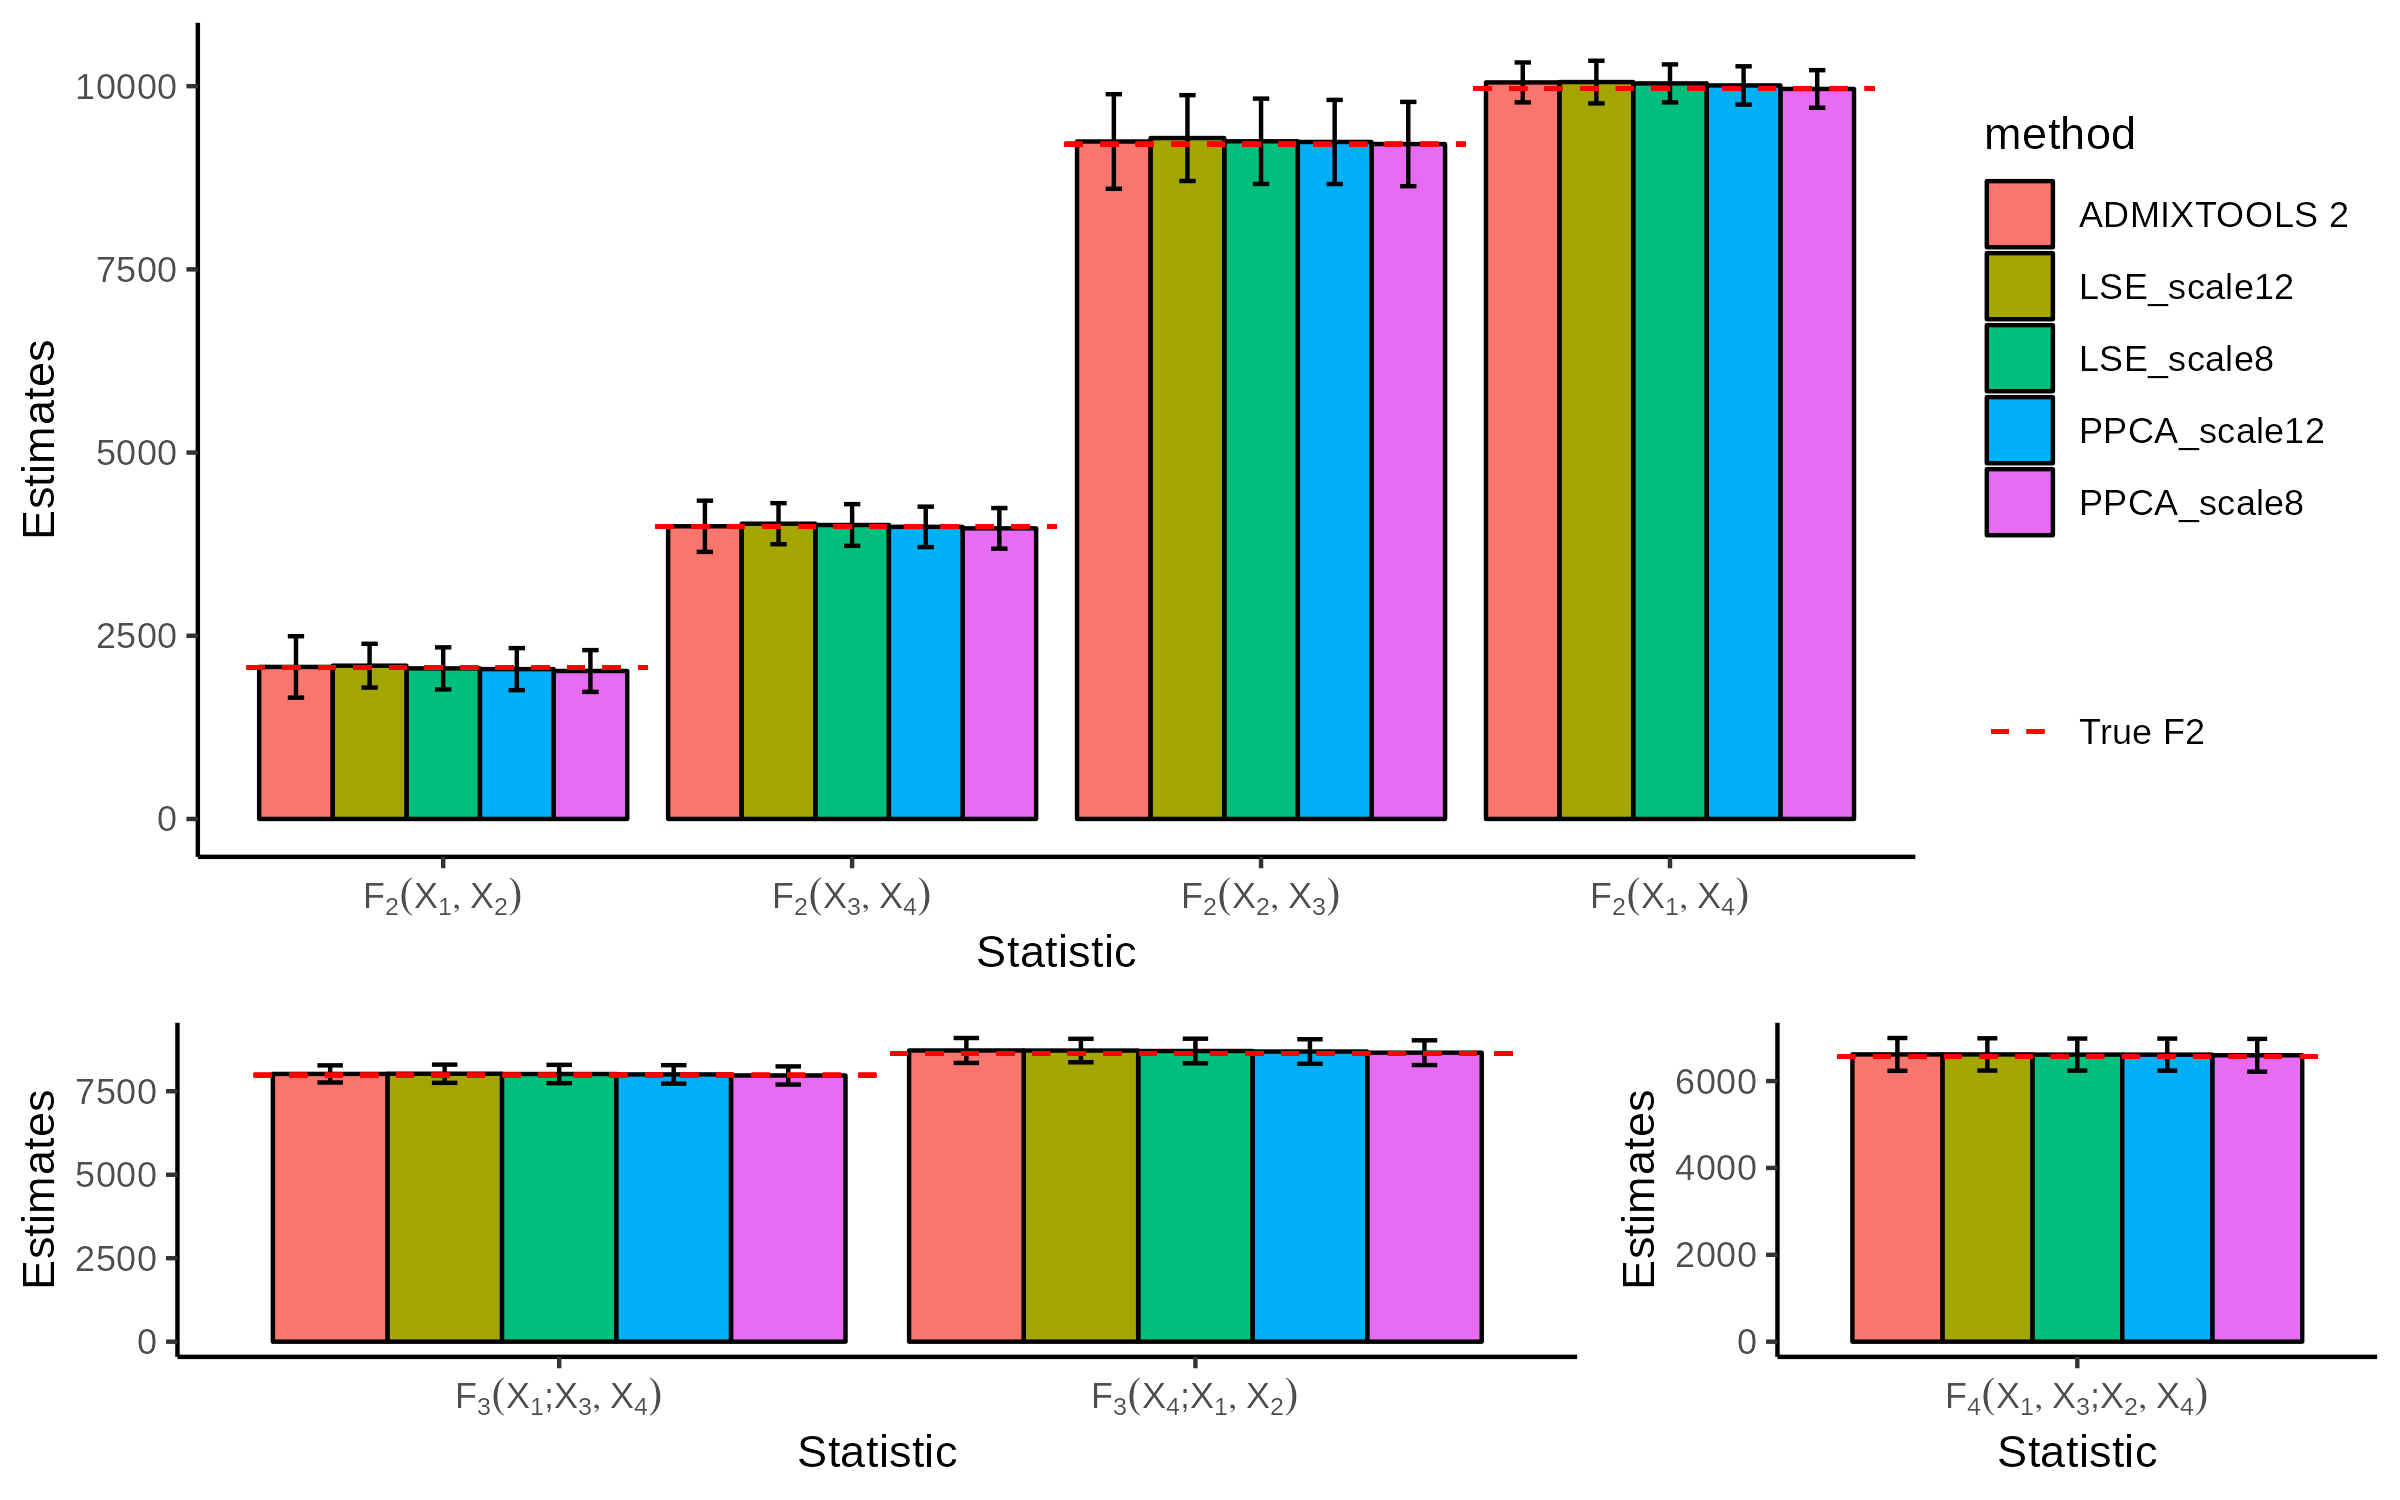
\includegraphics[width=16.5cm]{plots/simfiles/Ne1000/split_times1000/npop10_nind100/plots_8_12/mu0.05_plot_all_1ind.png}
    \centering
    \caption{Comparison of PPCA and LSE to ADMIXTOOLS 2 using population genotypes from one individual from each population.}
    \label{figS2:pc_scale}
\end{figure}

\begin{figure}[ht!]
    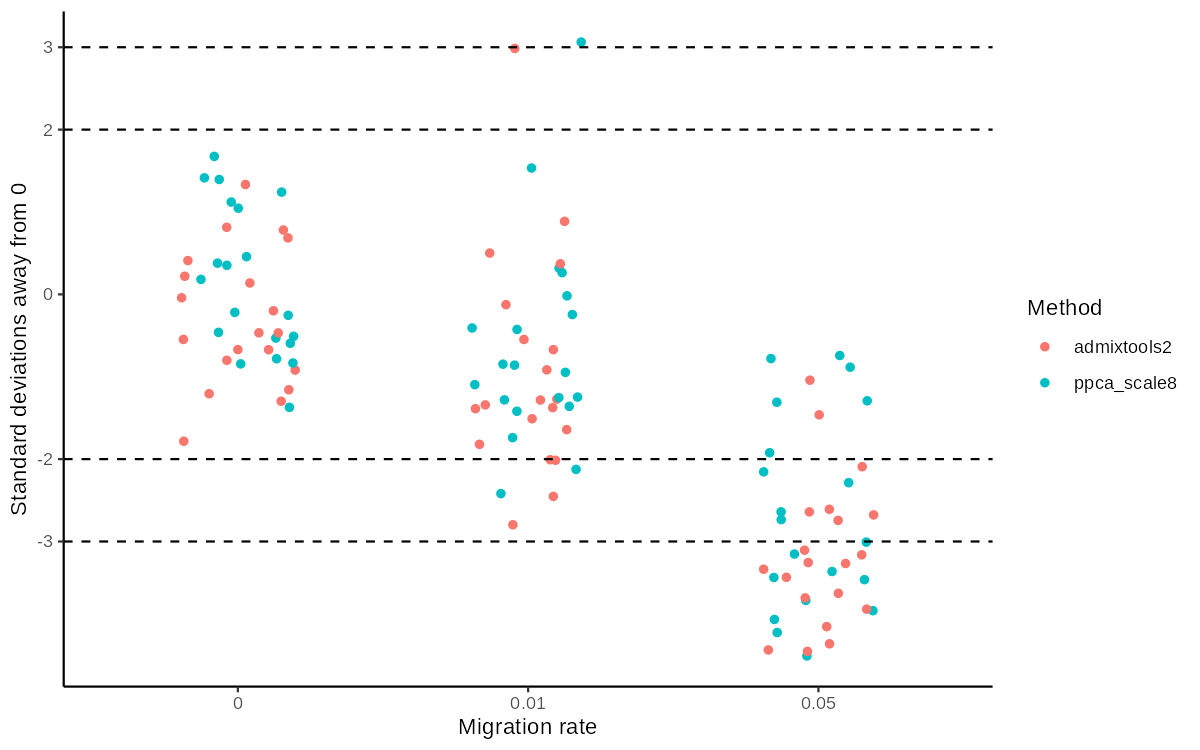
\includegraphics[width=16.5cm]{plots/simfiles/AvgFolder/Ne1000/split_times1000/npop10_nind100/missing0/plots_8/hypothesis_test_comparison.png}
    \centering
    \caption{Test for admixture with F4 statistic. We compare ADMIXTOOLS 2 (orange)to PPCA-based-framework (blue).}
    \label{figS2:pc_scale}
\end{figure}


\begin{figure}[ht!]
    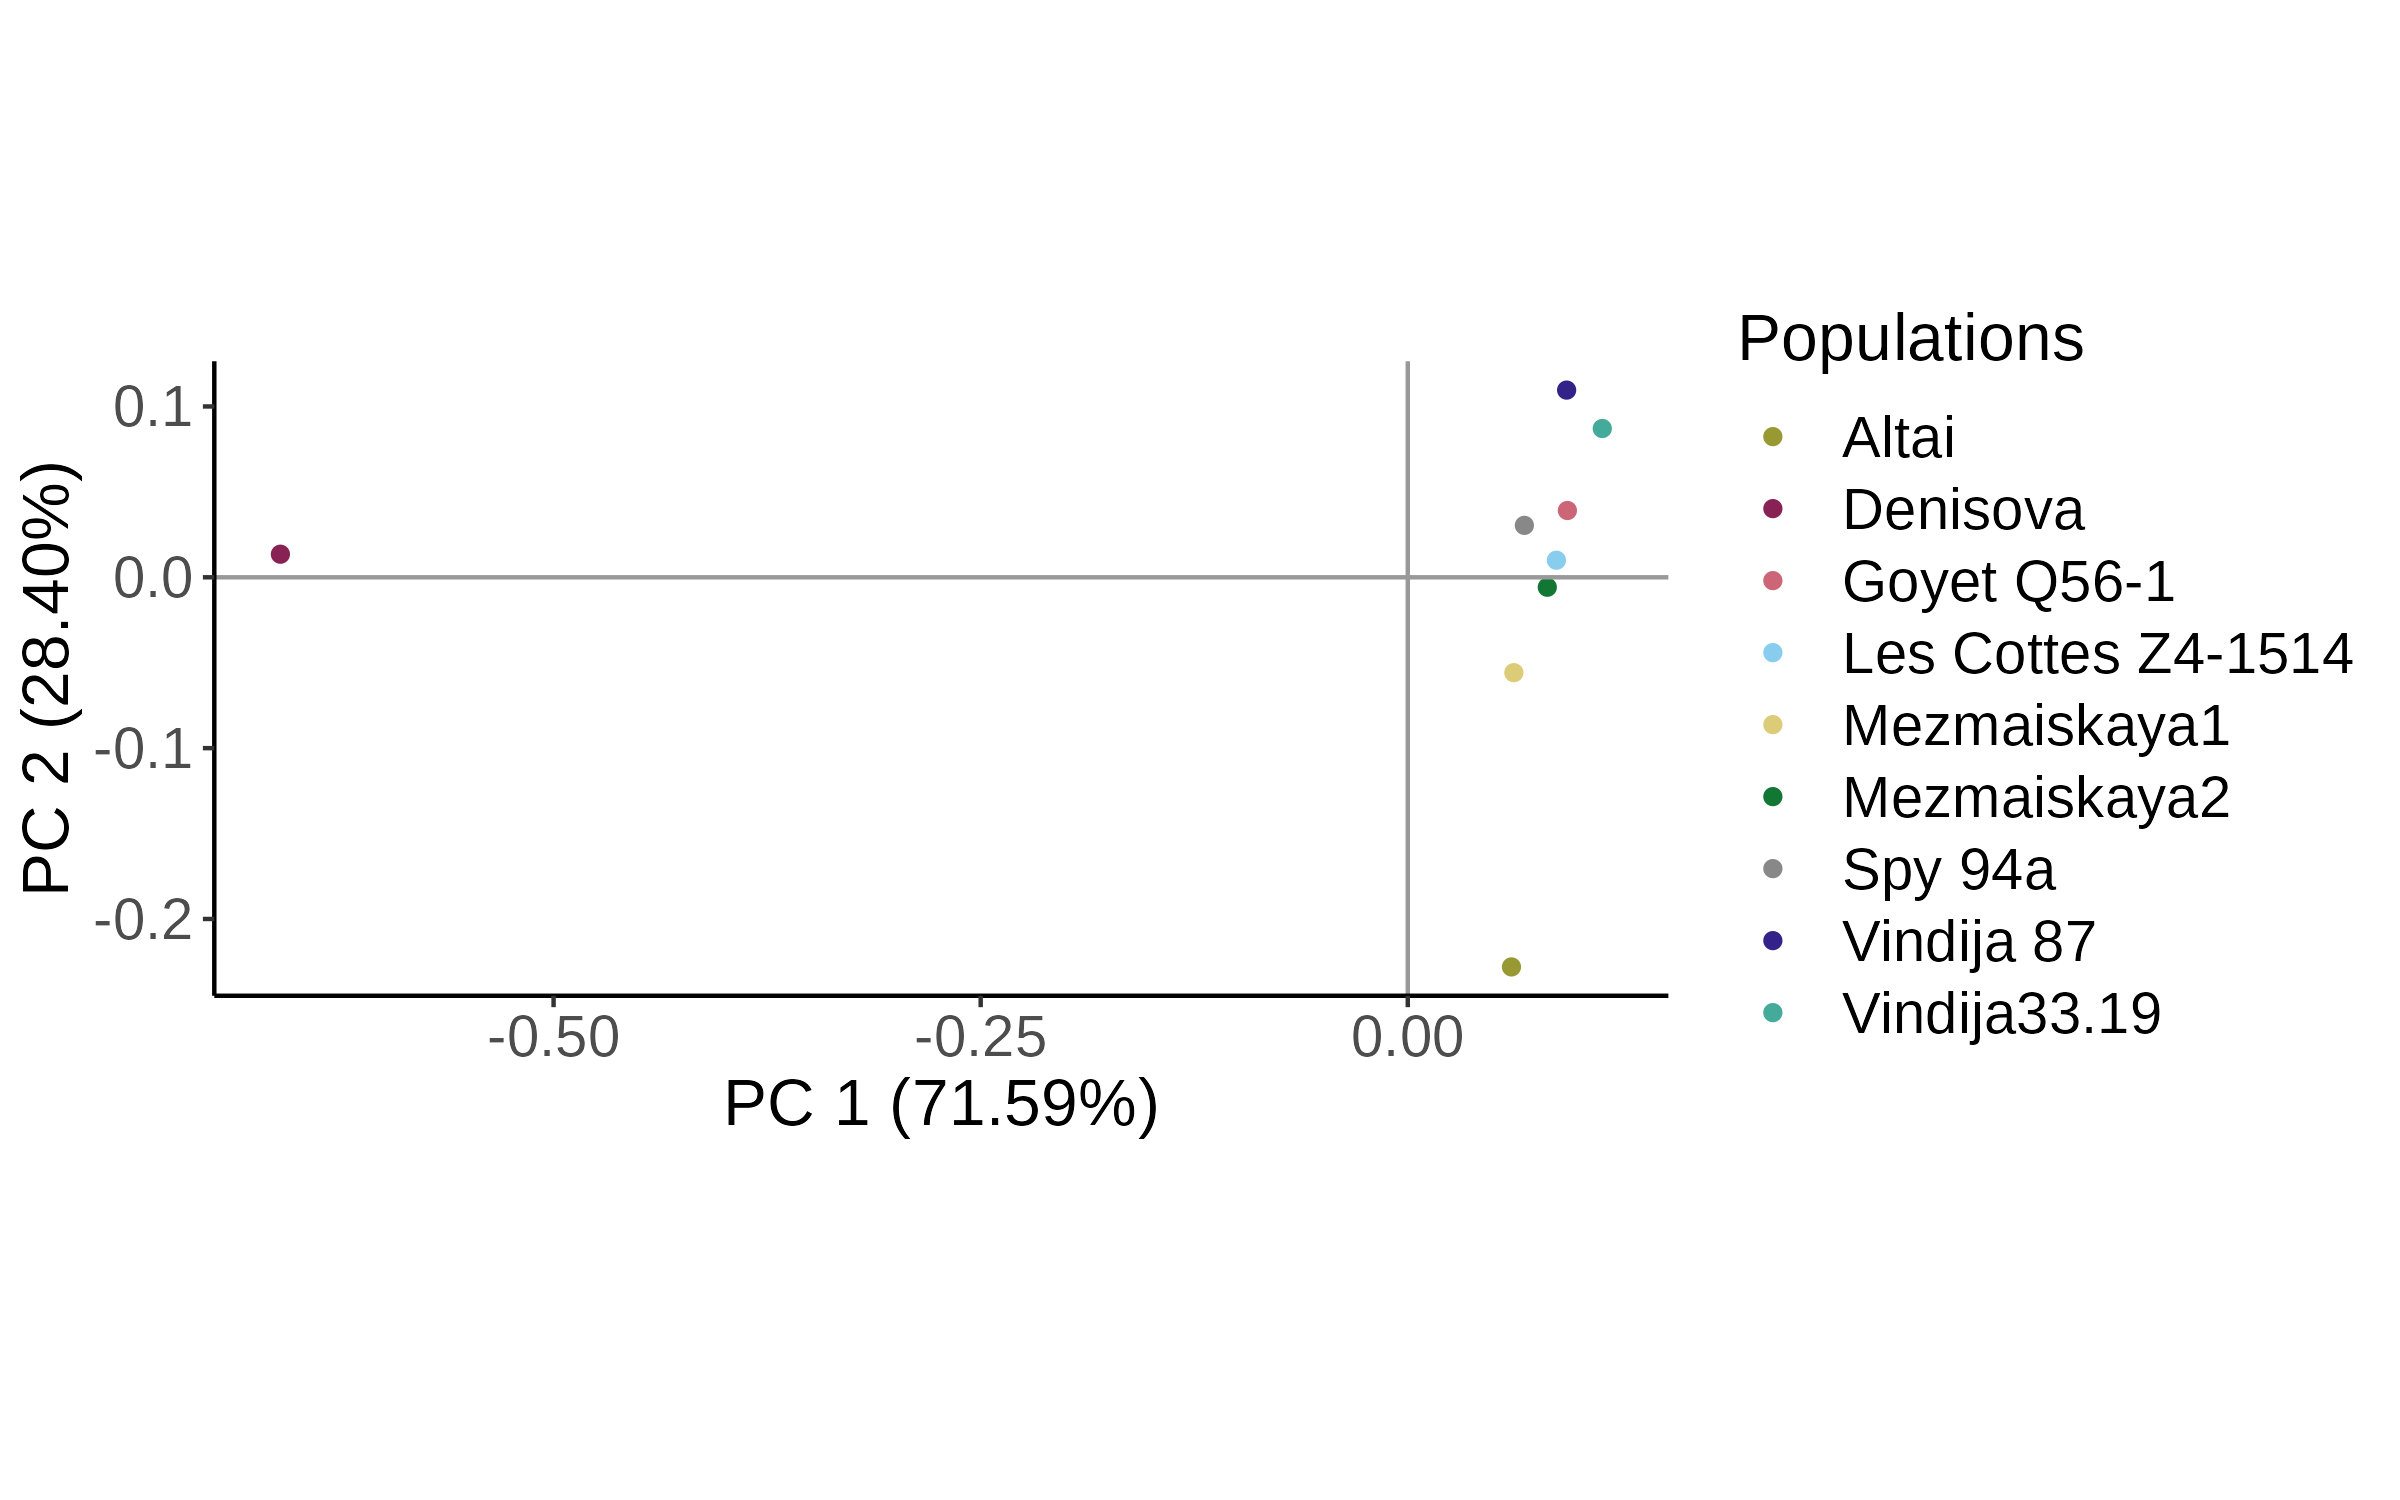
\includegraphics[width=16.5cm]{plots/neandertal_ppca.png}
    \centering
    \caption{PPCA of archaic specimens with scale=2.}
    \label{figS:ppca_nea}
\end{figure}

\begin{figure}[ht!]
    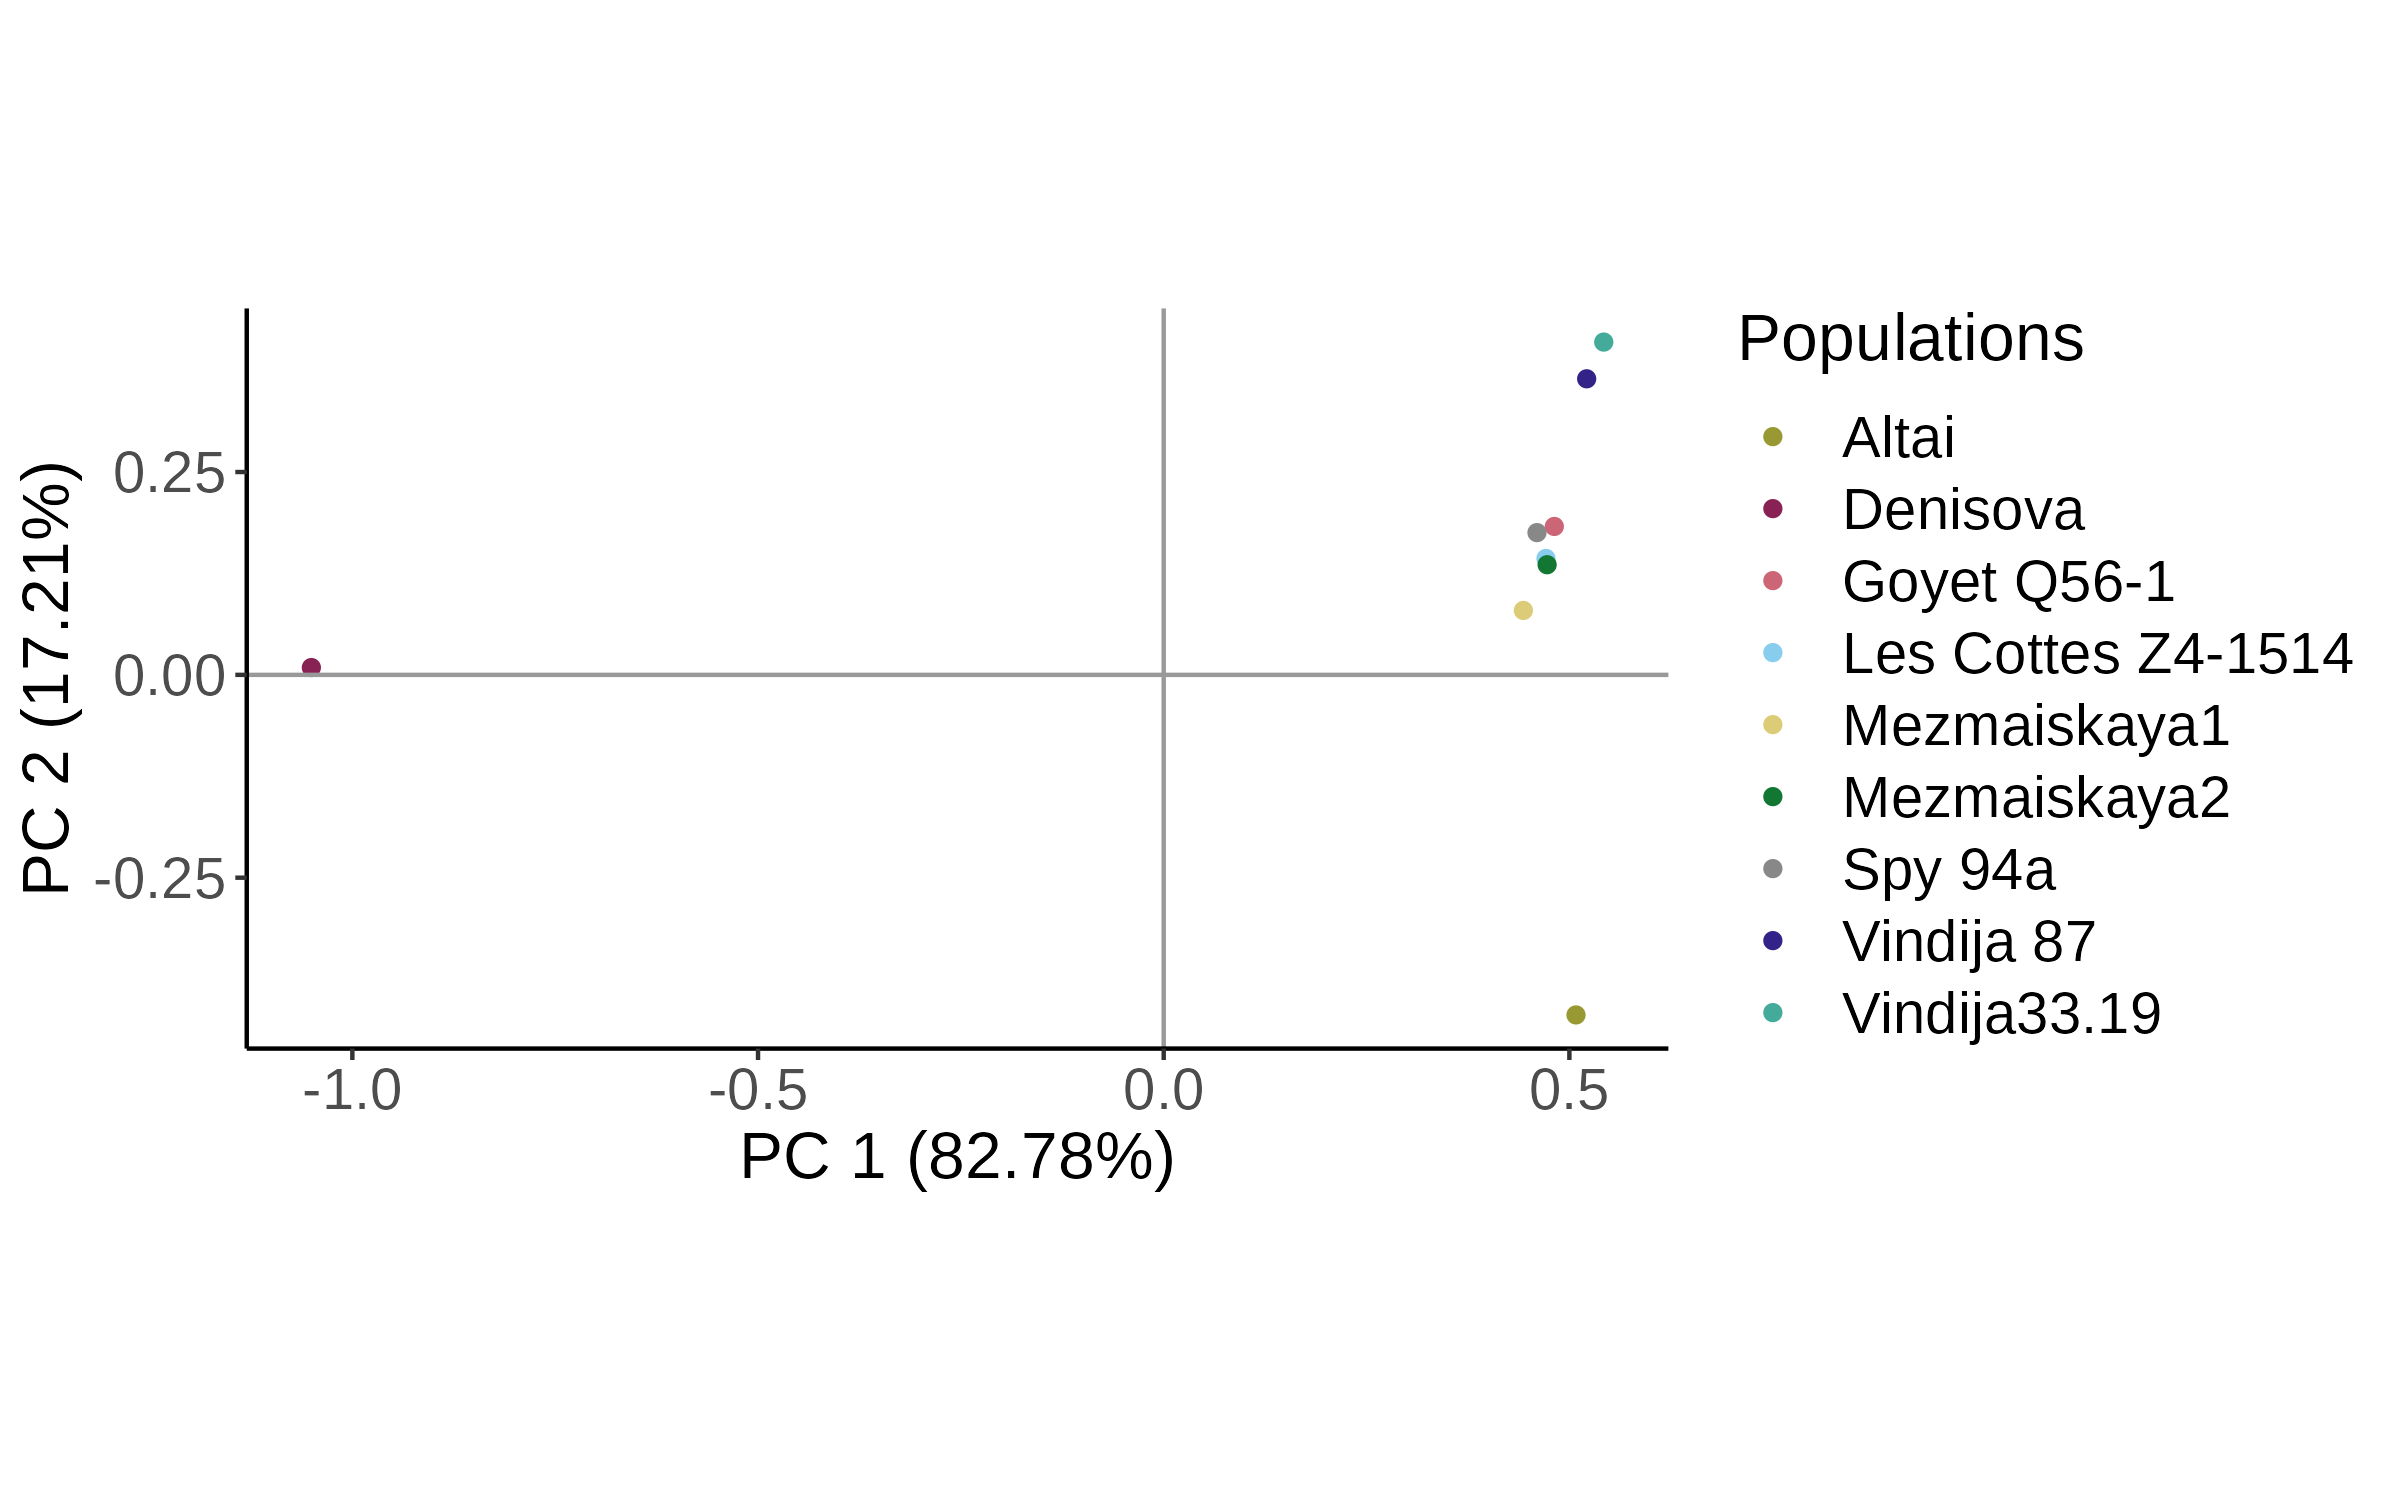
\includegraphics[width=16.5cm]{plots/neandertal_pca_smartpca.png}
    \centering
    \caption{PCA of archaic neandertals created with smartpca with high coverage neandertals, and projection of the rest. We used numoutevec=2 option to keep our analysis same as the authors \cite{mateja}.}
    \label{figS:smartpca_nea}
\end{figure}


\iffalse
\begin{figure}[ht!]
    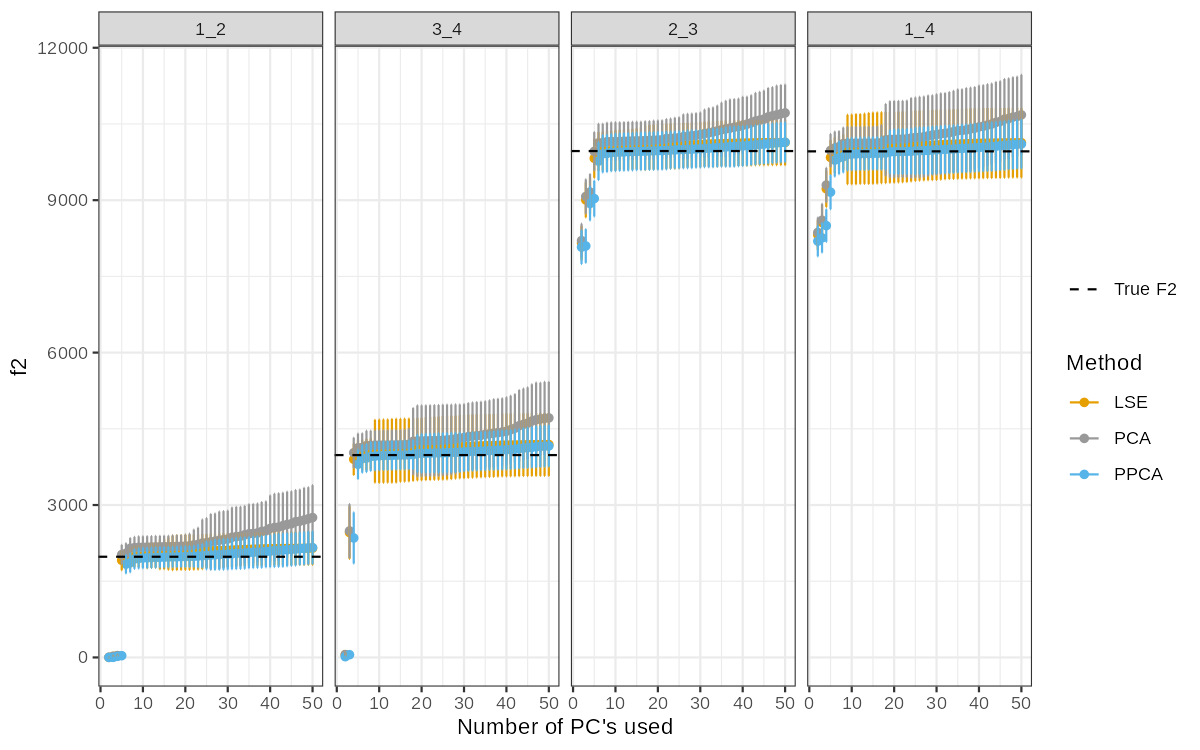
\includegraphics[width=16.5cm]{plots/supplementary/Ne1000_split_times1000_npop10_nind100_mu0_f2_plot_scale_test_ind.png}
    \centering
    \caption{Comparison of PCA, PPCA and LSE using population allele frequencies of 10 individuals in each population. X-axis shows the number of PC's used for the three methods, ranging from 2 to 50.}
    \label{figS1:pc_scale}
\end{figure}


\begin{figure}[ht!]
    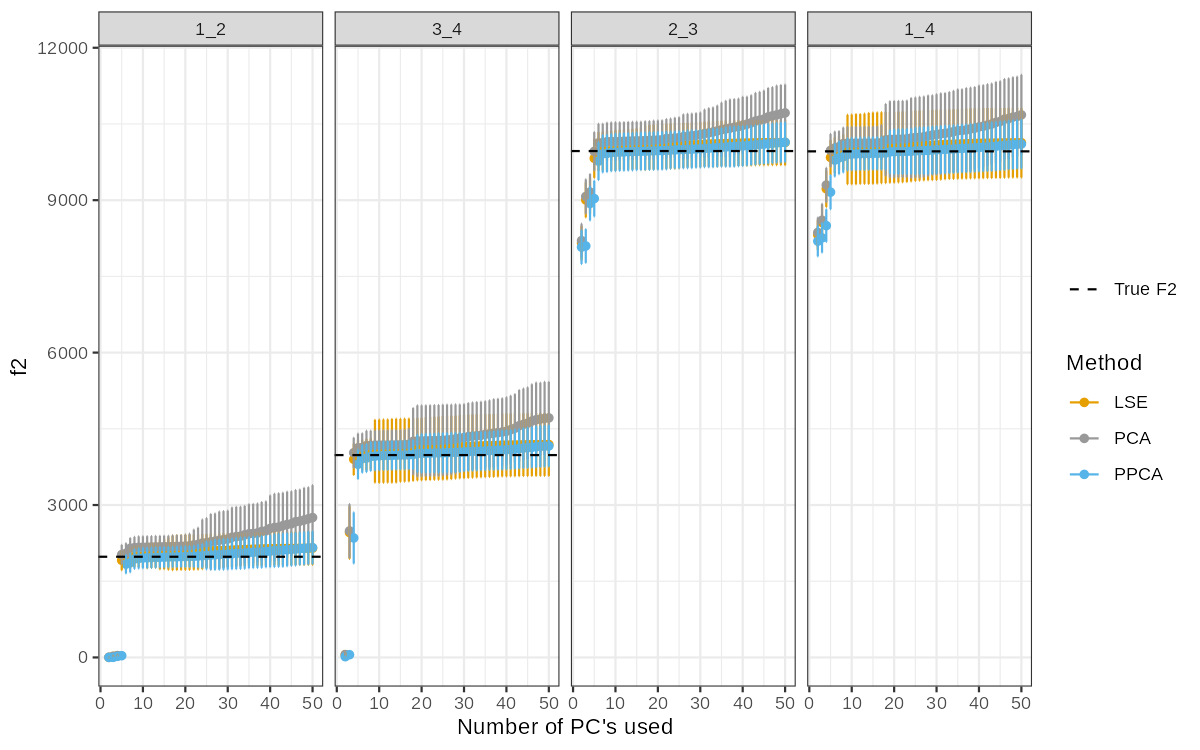
\includegraphics[width=16.5cm]{plots/supplementary/Ne1000_split_times1000_npop10_nind100_mu0_f2_plot_scale_test_ind.png}
    \centering
    \caption{Comparison of PCA, PPCA and LSE using population genotypes from one individual in each population. X-axis shows the number of PC's used for the three methods, ranging from 2 to 50.}
    \label{figS2:pc_scale}
\end{figure}
\fi




\end{document}